\documentclass{article}
\usepackage{amsmath,graphicx,amssymb,amsthm,url,listings}

\newcommand\tab[1][1cm]{\hspace*{#1}}

\title{Implementation Assignment 2}
\date{\today}
\author{Rong Yu and Finn Womack}

\begin{document}
	\maketitle
	\section*{Part 1: Loading Data and Implementing Gradient Batch}
After loading the testing and training data into feature and response matrices we implemented the batch gradient decent algorithm with the following learning rates:
	
	\begin{align}
		Rates &= \begin{bmatrix}
			2 \cdot 10^{-6} \\
			1 \cdot 10^{-6} \\
			3 \cdot 10^{-7} \\
			2 \cdot 10^{-7} \\
			1 \cdot 10^{-7} \\
		\end{bmatrix}
	\end{align}
	
	Then after running the algorithm on the above rates we plotted the iterations onto the loss function to get a sense of the convergence rate for the different learning rates:
	
	\newpage
	
	\begin{figure}[h!]
		\begin{center} 
			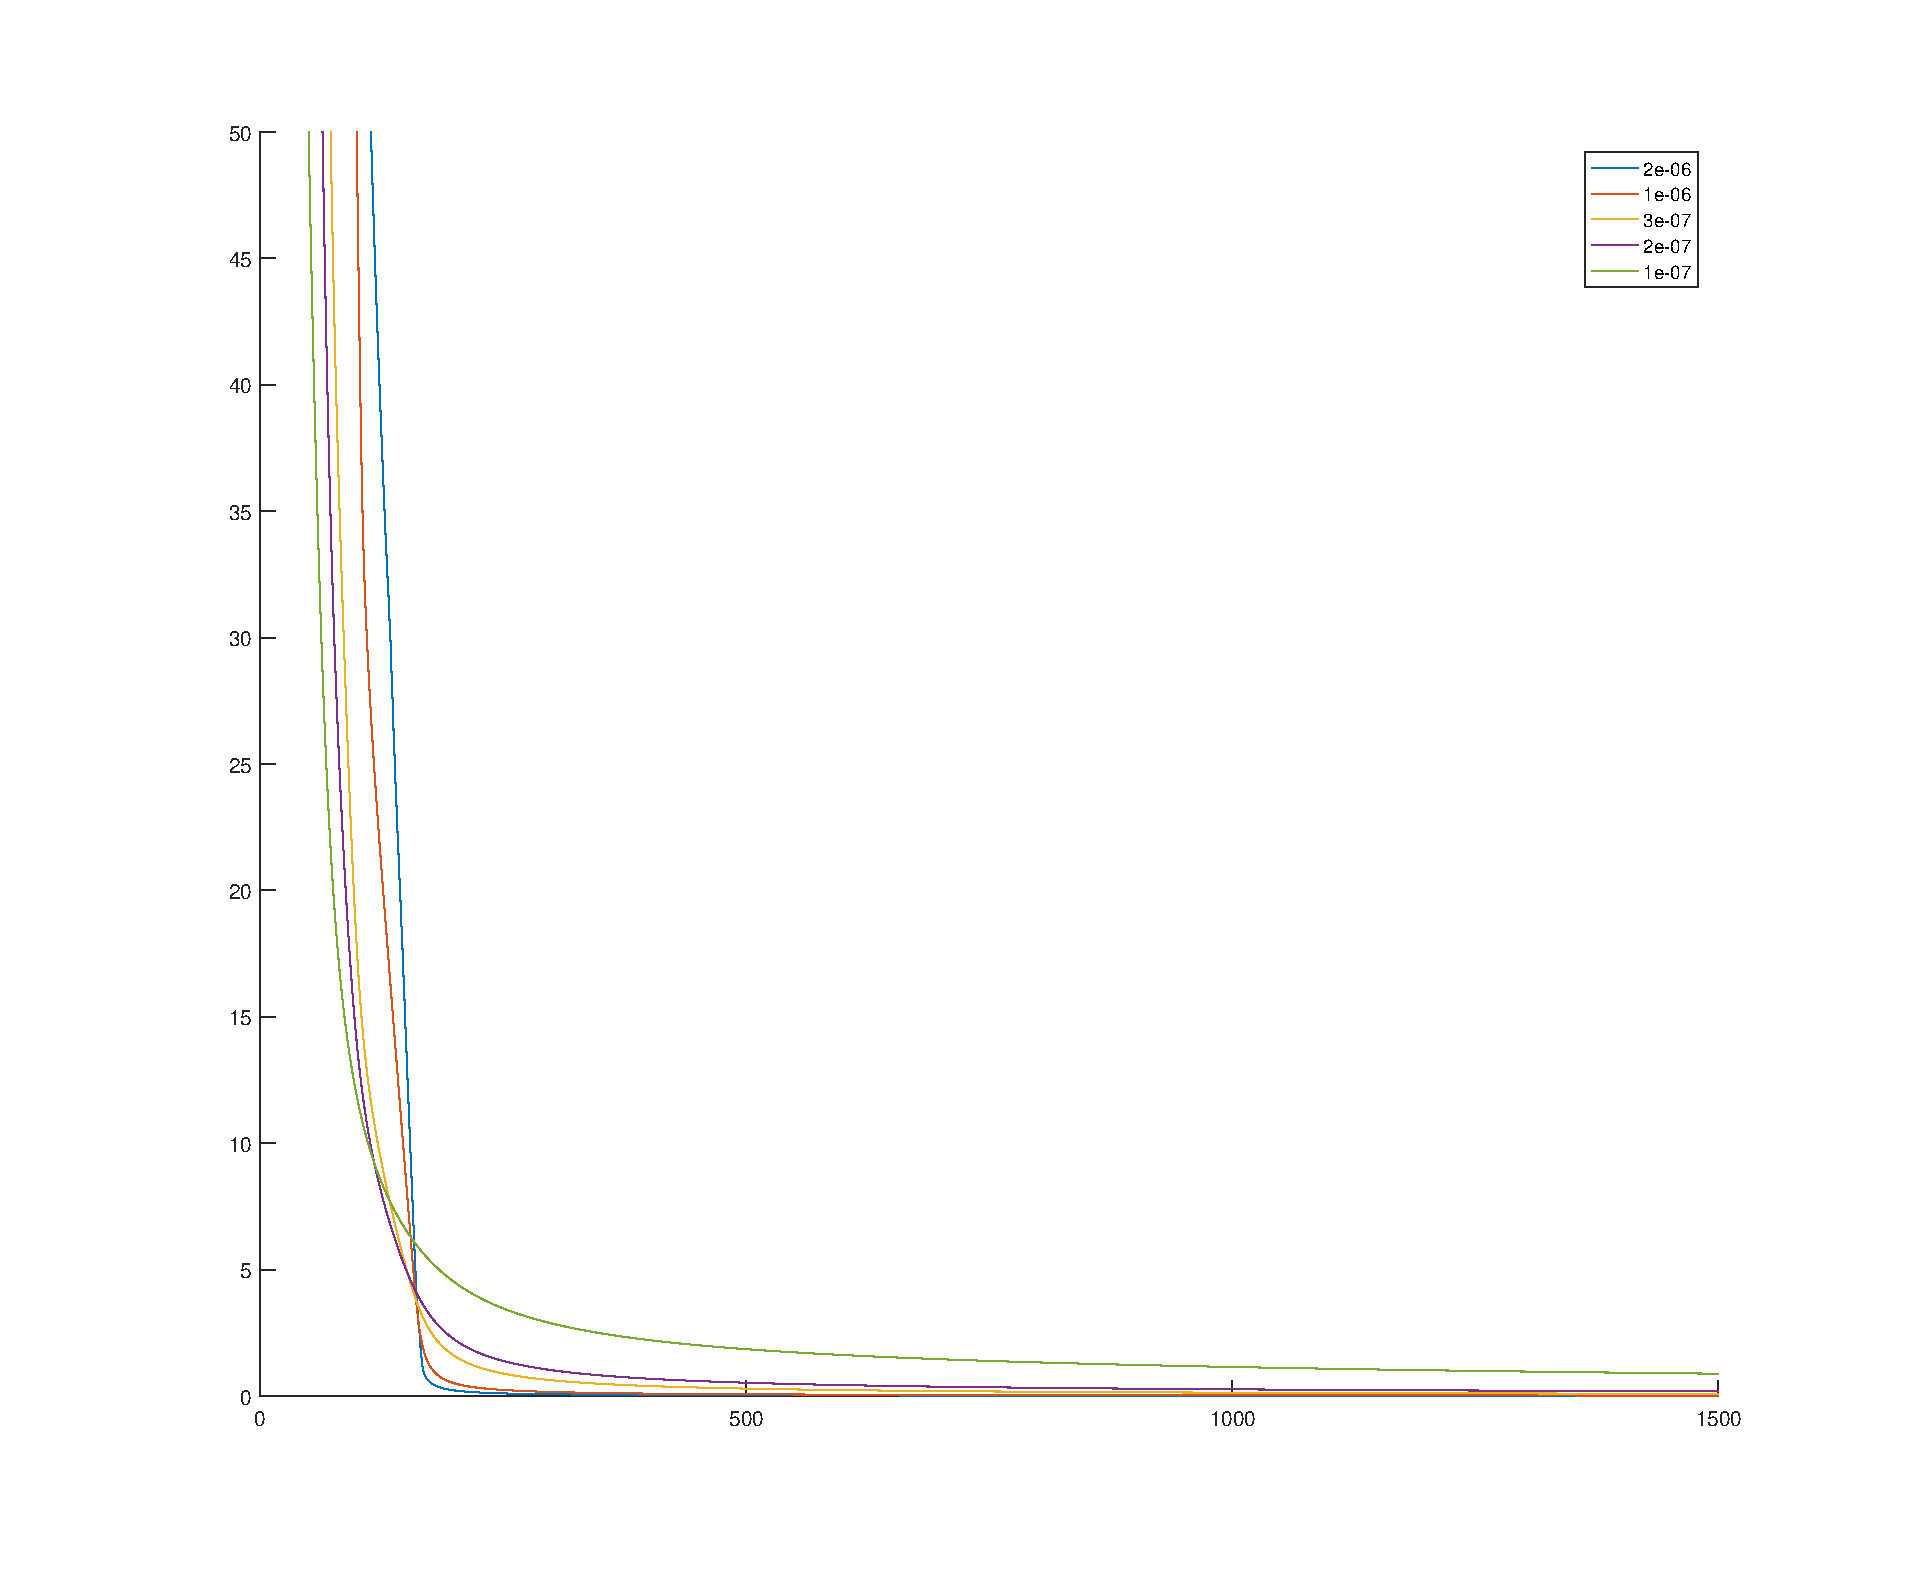
\includegraphics[scale=0.5]{learn_rates.eps} 
		\end{center} 
		\label{fig:M1}
	\end{figure}
	
	The learning rate of $2 \cdot 10^{-6}$ gives the fastest convergence. When we picked larger learning rates we started to get oscillations.
	
	\section*{Part 2: Testing and Training Accuracies}
	
	We then selected the learning rate of $1 \cdot 10^{-7}$ to test the effects of iterations on the testing and training accuracies:
	\newpage
	
	\begin{figure}[h!]
		\begin{center} 
			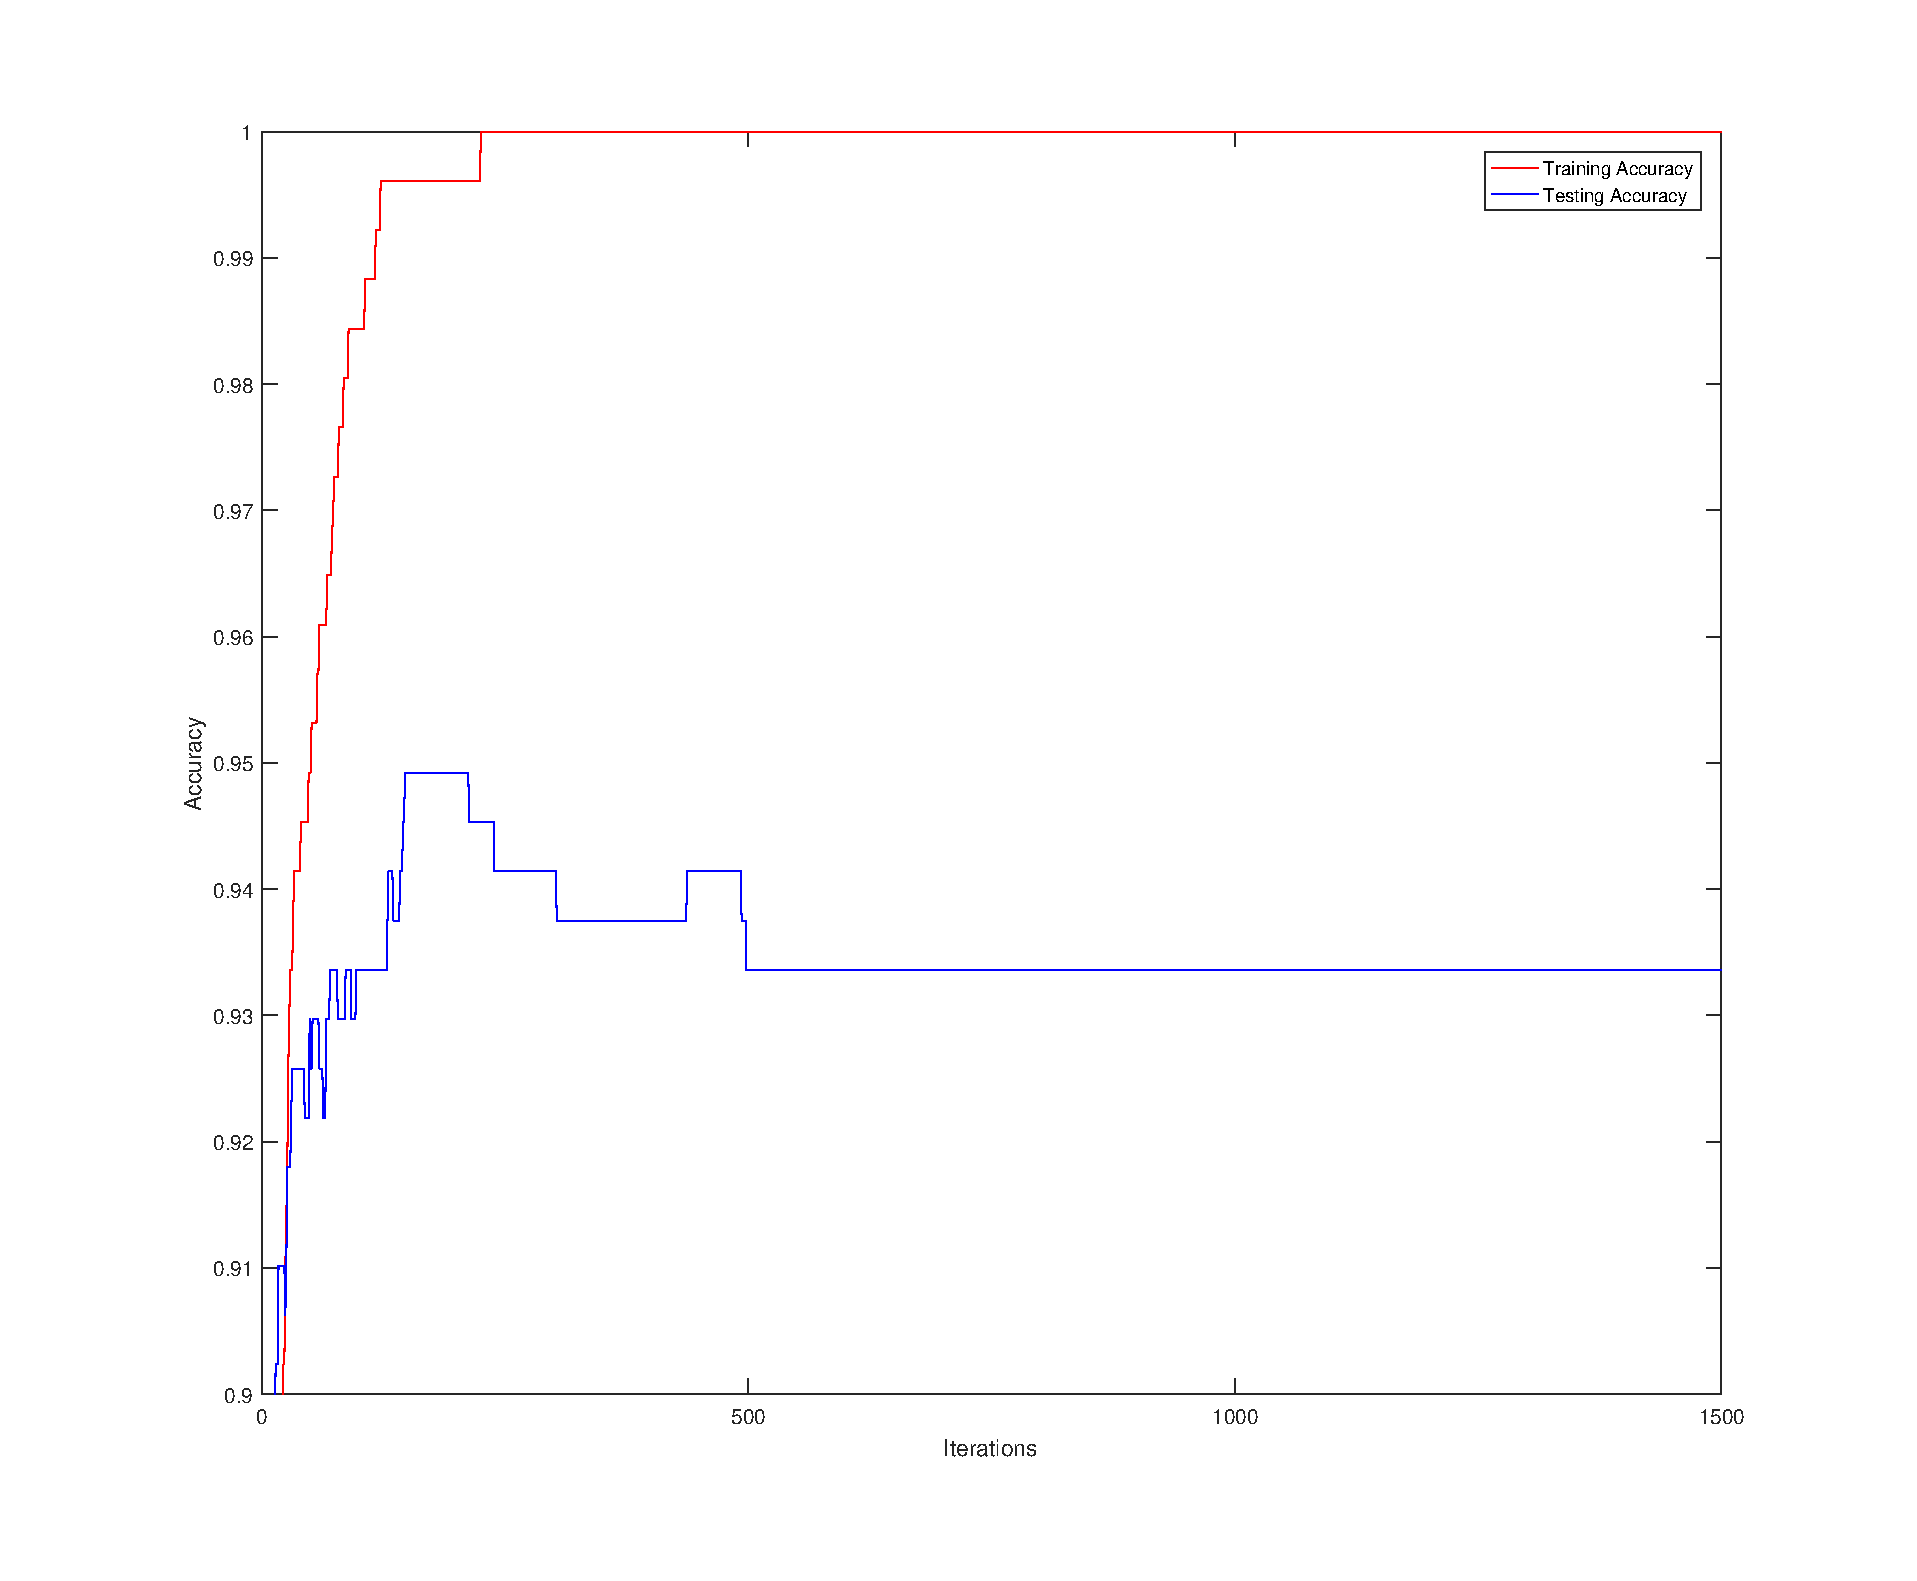
\includegraphics[scale=0.5]{iter_accuracy.eps} 
		\end{center}  
		\label{fig:M2}
	\end{figure}

As we can see the training accuracy converges to 1 and the testing accuracy peaks at around 175 iterations and then decreases.

	\section*{Part 3: Deriving the Regularization Term}
Consider the new objective function:
	
	$$
	L(w) = \sum_{i = 1}^{n} l(w^{T} x_{i}, y_{i}) + \frac{\lambda}{2} \Vert W \Vert_{2}^{2}
	$$
	
	This is the the same as the original objective function with an added term and since the gradient of a sum of functions in the sum of the gradients all we need to do is find the gradient of $\frac{\lambda}{2} \Vert W \Vert_{2}^{2}$:
	
	\begin{align}
	\nabla \frac{\lambda}{2} \Vert W \Vert_{2}^{2} &= \frac{\lambda}{2} \nabla \Vert W \Vert_{2}^{2} \\
	 &= \frac{\lambda}{2} \nabla \sum_{i = 1}^{m} w_{i}^{2} \\
	 &= \frac{\lambda}{2} \begin{bmatrix}
		 \frac{\partial}{\partial w_{1}} \sum_{i = 1}^{m} w_{i}^{2} \\ \\
		 \frac{\partial}{\partial w_{2}} \sum_{i = 1}^{m} w_{i}^{2} \\
		 \vdots \\
		 \frac{\partial}{\partial w_{m}} \sum_{i = 1}^{m} w_{i}^{2} \\
		 \end{bmatrix}\\
	&= \frac{\lambda}{2} \begin{bmatrix}
	2 w_{1} \\
	2 w_{2} \\
	\vdots \\
	2 w_{m} \\
	 \end{bmatrix}\\
	&= \lambda W
	\end{align}
	
Thus the new batch gradient code would be as follows:\\
Given: training examples $(x_{i}, y_{i}), i = 1, ..., N$ \\
$W \leftarrow [0, 0, ..., 0]$ \\
Repeat until convergence: \\
\tab $ d \leftarrow [0, 0, ..., 0]$ \\
\tab For i = 1 to N do \\
\tab \tab $\hat{y}_{i} \leftarrow \frac{1}{1 + e^{-w \cdot x_{i}}}$ \\
\tab \tab $error = y_{i} - \hat{y}_{i}$ \\
\tab \tab $d = d + error \cdot (x_{i} + 2 w)$ \\
\tab $w \leftarrow w + \eta d$
		


	
	\section*{Part 4: Implementing Regularization}
	
To examine the effect of regularization on the algorithm we plotted the testing and training accuracies against the following choices of $\lambda$:
	
	\begin{align}
		\lambda \begin{bmatrix}
		10^{-6} \\
		10^{-4} \\
		10^{-2} \\
		1 \\
		10^{2} \\
		10^{4} \\
		10^{6}
		\end{bmatrix} 
	\end{align}
	
The resulting plot is as follows:

	
	\begin{figure}[h!]
		\begin{center} 
			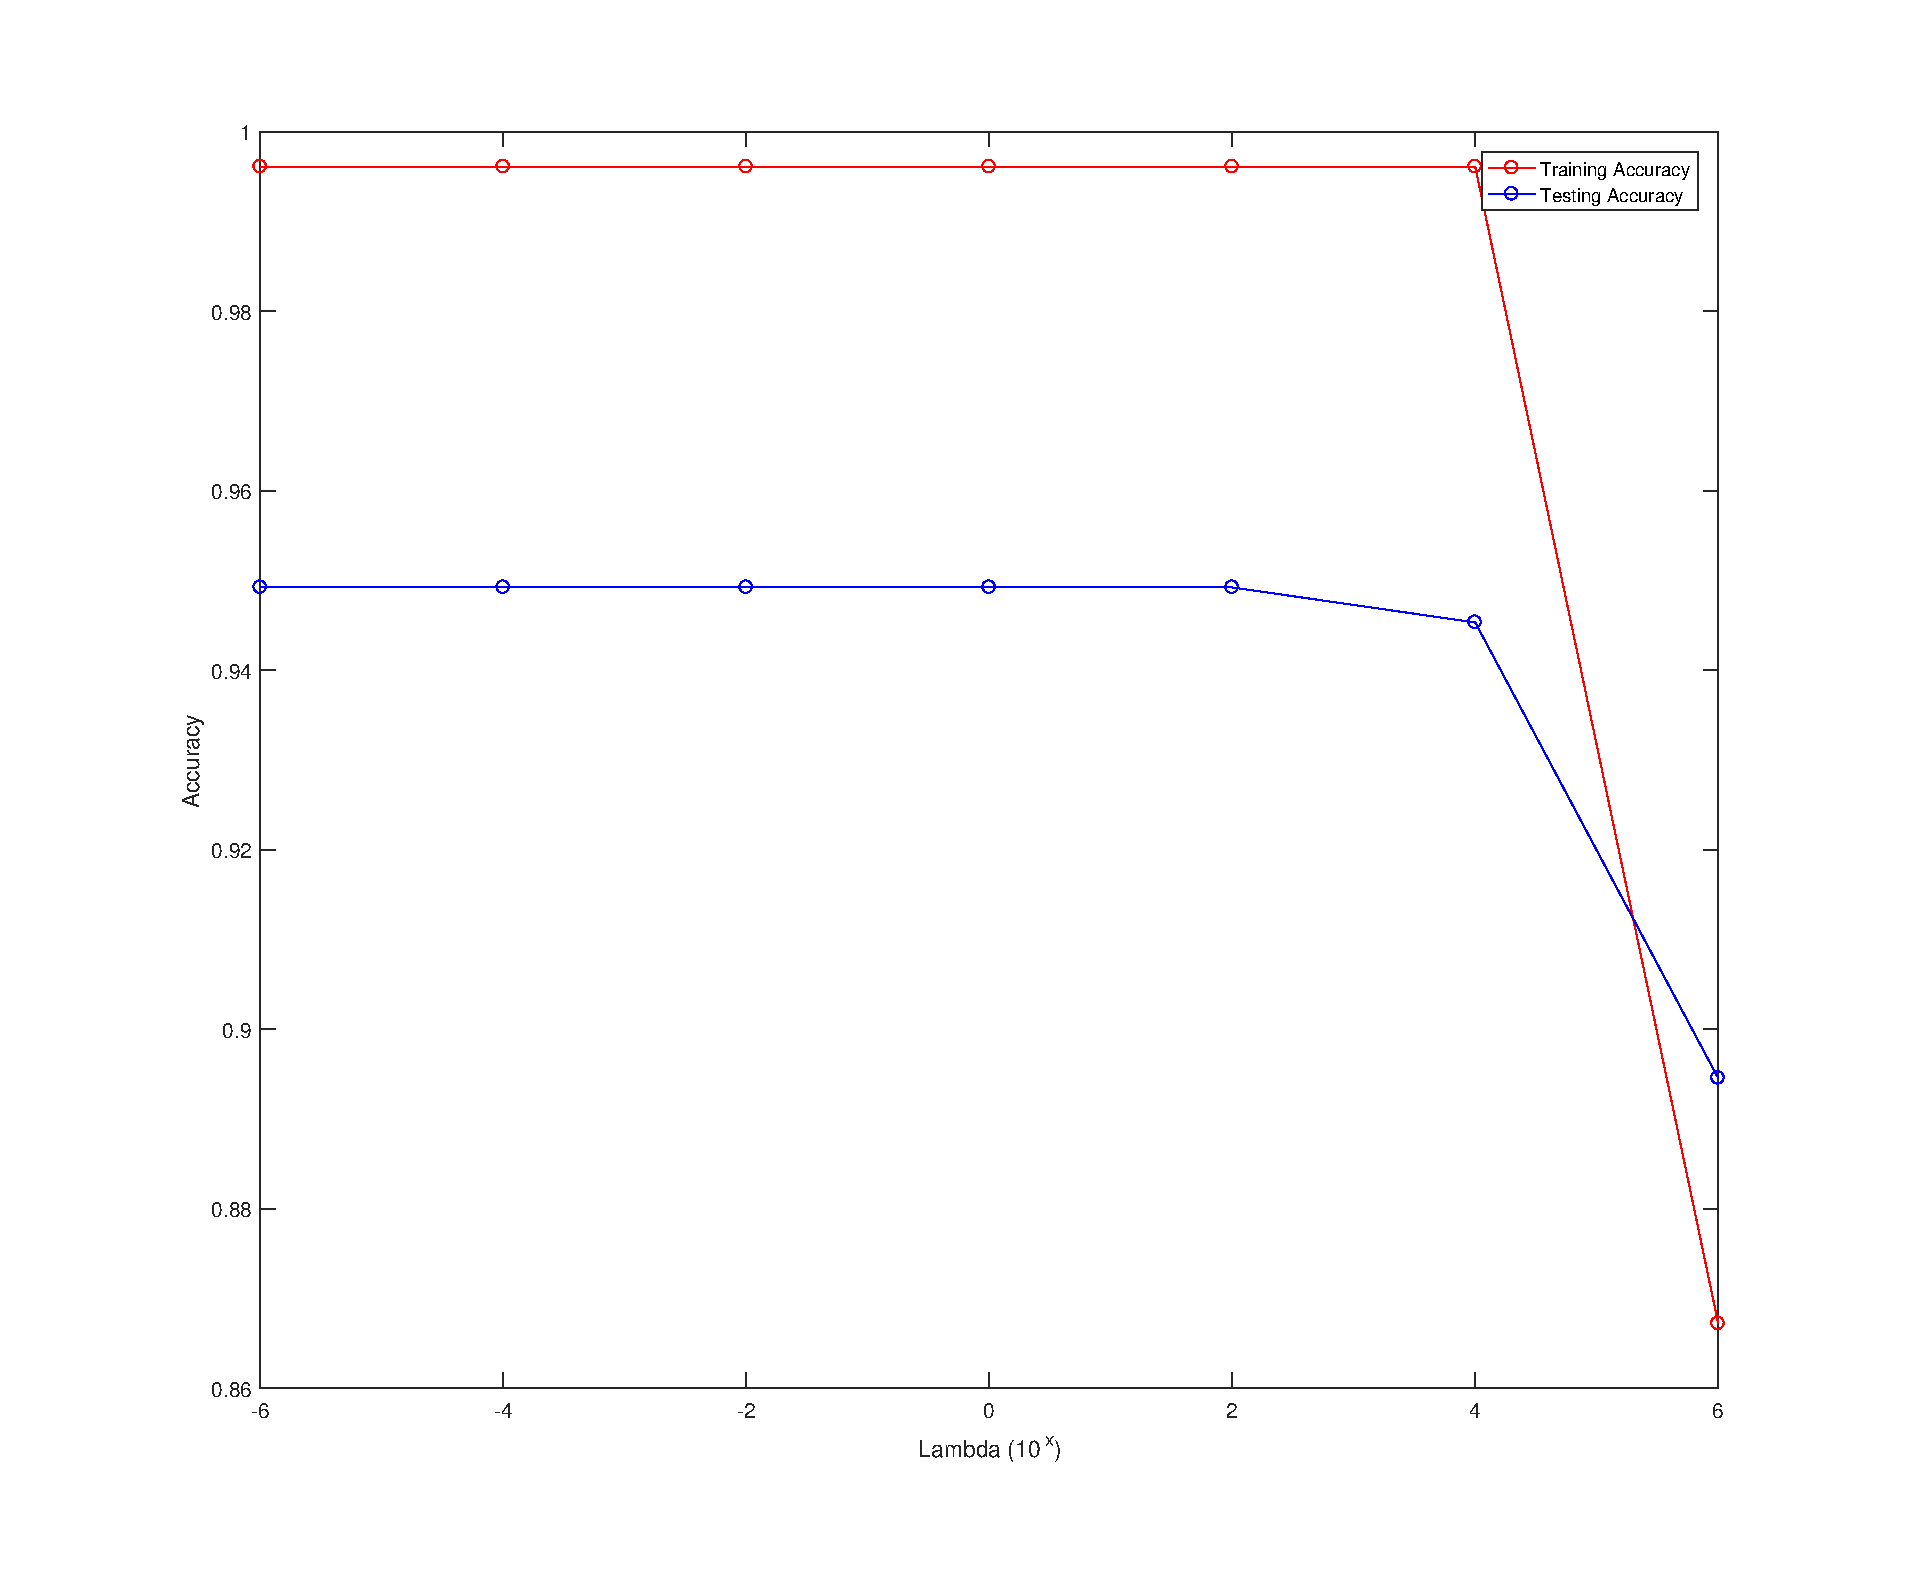
\includegraphics[scale=0.5]{lambda_accuracy.eps} 
		\end{center}  
		\label{fig:M3}
	\end{figure}
\newpage


	
	%\bibliography{myCitations} 
	%\bibliographystyle{abbrv}
	
\end{document} 